\renewcommand{\theauthor}{Dario Wagner}
\justifying
\section{Parser}
\label{sec:parser}
\subsection{Aufgabe}
\label{sec:parser-aufgabe}
Die Aufgabe des Parsers ist es auf die Datenbank zuzugreifen und sich die, für das iCal Format notwendigen, Daten zu holen. Diese werden anschließend vom Parser in einen iCal String umgewandelt, damit der benutzte Kalender diesen verwerten kann und passende Termine erstellt. 

\subsubsection{Source-Code}
\label{sec:parser-sourcecode}
Unter dieser Überschrift wird auf einen wichtigen Teil des Parsers eingegangen um seine Funktionsweise in Kombination mit dem Entity Framework zu verstehen. Im Prinzip besteht der Parser aus zwei Teilen, dem Verbindungsaufbau mit der Datenbank(DB) über das Entity Framework und dem konvertieren der Daten zu einer iCal-Zeichenkette. Da der zweite Teil sich nur mit reinem Abfragen ob Daten vorhanden sind und wenn sie vorhanden sind dem hinzufügen zum StringBuilder beschäftigt wird dieser Teil nicht erklärt.\\ \\
Im folgenden eingefügten Source-Code ist zu sehen wie man mit hilfe des Parser auf die Datenbank zugreifen kann. Der Source-Code ist anhand von Kommentaren in vier Parts aufgeteilt. Das Source-Code Beispiel wurde identisch aus dem praktischen Teil der Diplomarbeit in der Klasse Parser unter der Methode GetICalFormat(int UserID) übernommen. \\ \\
\textbf{Part 1} \\
Im ersten Part wird der StringBuilder, welcher letzten Endes die fertige Zeichenkette zurückgibt, erstellt. Anschließend wird über den ''using''-Command [\ref{usingkeyword}] ein Objekt mit dem Namen ''db'' von der Klasse iCalContext erstellt. Die Klasse iCalContext wurde vom Entity Framework automatisch generiert und wird unter folgender Überschrift ''\ref{ef-sourcecode} Source-Code'' erklärt. Unter dem Schlüsselwort ''using'' wird desweiteren eine Boolean-Variable erstellt, welche später bei einer Abfrage benötigt wird. Diese kann vorerst ignoriert werden, da sie für die Erklärung irrelevant ist. Im Anschluss wird eine Liste des Typen ''int'' erstellt, welche später unsere Kalender-IDs enthalten wird. \\ \\
\textbf{Part 2} \\
In diesem Abschnitt wird über eine foreach-Schleife durch eine Liste iteriert welche alle Calender IDs enthält die dem übergebenem User gehören. In der Schleife werden alle IDs in die CalendarIdList gespeichert. \\ \\
\textbf{Part 3} \\
In Part 3 ist der Kopf der foreach-Schleife die sich bis zum Ende der Methode durchzieht zusehen. In dieser werden alle Kalender, mit einer ID, welche in der CalendarIdList enhalten sind, iteriert. Das heißt die Methode wird erst beendet wenn alle Kalender des Benutzers in einen iCal-String umgewandelt wurden und im StringBuilder enthalten sind. Da am Anfang von jedem Kalender immer ''BEGIN:VCALENDER'' und eine Timezone angegeben wird, wird dieser String direkt an den StringBuilder angehängt. \\ \\
\textbf{Part 4} \\
In Part 4 sieht man den Kopf einer foreach-Schleife welcher dafür sorgt, dass durch jeden Termin oder Eintrag im Kalender durchiteriert wird. Da das iCal-Format für einen Kalender wie folgt aufgebaut ist: 
\begin{itemize}
\item Kalender Anfang
\item Termin/Eintrag
\item ...
\item Kalender Ende
\end{itemize}

\begin{lstlisting}[caption=Parser Verbindung zur DB mit dem Entity Framework, label=lst:test]
// Part 1
StringBuilder iCalFormat = new StringBuilder();
using (var db = new iCalContext())
{
  bool isTodo = false;
  List<int> CalendarIdList = new List<int>();
  // Part 2
  foreach (var userhascal in db.UserHasCalendar.Where
  		  (y => y.UserId == UserID))
  {
	CalendarIdList.Add(userhascal.CalendarId);
  }
  // Part 3
  foreach (var calendar in db.Calendar.Where
  		  (x => CalendarIdList.Contains(x.CalendarId)))
  {
    iCalFormat.Append("BEGIN:VCALENDER\nVERSION:2.0\nMETHOD:PUBLISH\n"
	+ "TZID:" + calendar.TimeZone.Continent + "-" 
    + calendar.TimeZone.Country + "\n");
    // Part 4
    foreach (var calendarEntry in calendar.CalendarEntry)
    {
\end{lstlisting} 
\paragraph{using-Schlüsselwort in C\#}
\label{usingkeyword}
Using wird verwendet wenn man sichergehen will, dass das Objekt oder die Objekte in using entsorgt werden. Um zu veranschaulichen wie using funktioniert, folgendes Beispiel.

\begin{lstlisting}[caption=Parser funktionsweise von using, label=lst:test]
// using Schluesselwort
using (MyResource myRes = new MyResource())
{
    myRes.DoSomething();
}
 
// Funktionsweise von using 
{ // Limits scope of myRes
    MyResource myRes= new MyResource();
    try
    {
        myRes.DoSomething();
    }
    finally
    {
        // Check for a null resource.
        if (myRes != null)
            // Call the object's Dispose method.
            ((IDisposable)myRes).Dispose();
    }
}
\end{lstlisting} 
\textcite{ParserUsingKeyword}
\subsection{Entity Framework}
\label{sec:parser-entity-framework}
\subsubsection {Funktionsweise}
Mithilfe des Entity Framework lässt sich eine Datenbankstruktur innerhalb des Projekts mit Klassen darstellen. Wenn auf eine dieser Klassen in Form einer Value-Abfrage zugegriffen oder durch sonstige GET/SET Methoden, wird durch das Entity Framework ein Datenbank Zugriff durchgeführt. 
Um die Funktionsweise genauer zu verstehen folgt ein Beispiel mit einer Datenbank in welcher Autos gespeichert werden:
HIER KOMMT DANN EIN BEISPIEL
\subsubsection {Anwendung}
Voraussetzung: Funktionsfähige ASP.NET Web Application \\
\break \textbf{1. Erstellung einer Datenbank} \\
Als Beispiel wurde für dieses Beispiel die Scott Tiger Datenbank verwendet.
\break \url{http://jailer.sourceforge.net/scott-tiger.sql.html} \\
\break \textbf{2. Installieren des EntityFrameworks} \\
In der Packet Manager Console folgenden Befehl eingeben und bestätigen: 
\begin{figure}[H]
	\centering
    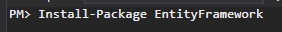
\includegraphics[width=0.5\textwidth]{Parser_EFUse01}
    \caption{Install}
    \label{fig:parsef01}
\end{figure}
Abschluss der Installation sieht wie folgt aus:
\begin{figure}[H]
    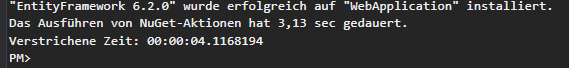
\includegraphics[width=0.9\textwidth]{Parser_EFUse02}
    \caption{Install complete}
    \label{fig:parsef02}
\end{figure} 

\textbf{3. Entity Framework generiert Klassen aus DB} \\
Im Solution Explorer auf den Model Ordner Rechtsklick machen -> ''Hinzufügen'' -> ''Neues Element''
\begin{figure}[H]
    \centering
    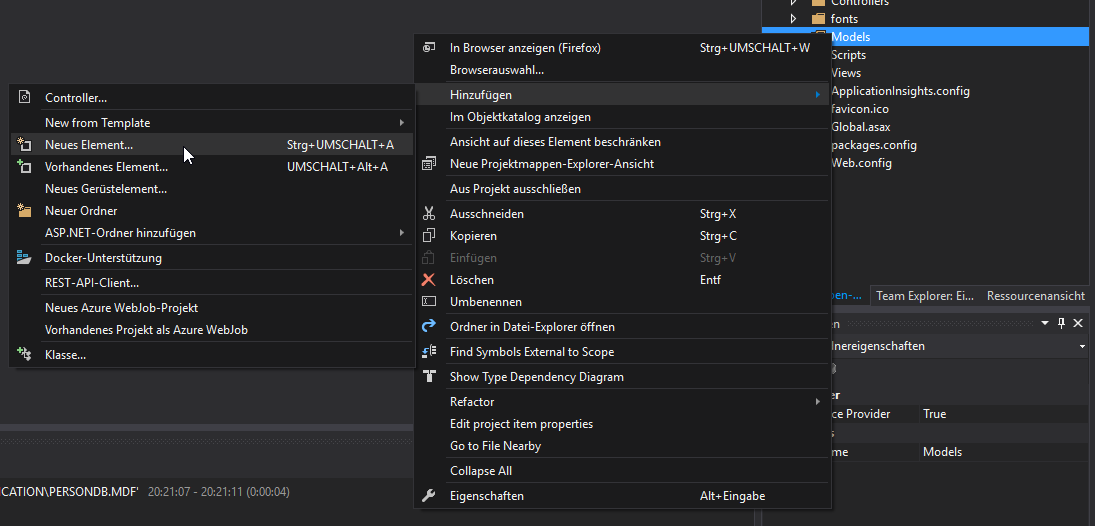
\includegraphics[width=\textwidth]{Parser_EFUse03}
    \caption{Neues Element}
    \label{fig:parsef03}
\end{figure} 
Anschließend auf ''Daten'' -> ''ADO.NET Entity Data Model'' -> Hinzufügen
\begin{figure}[H]
    \centering
    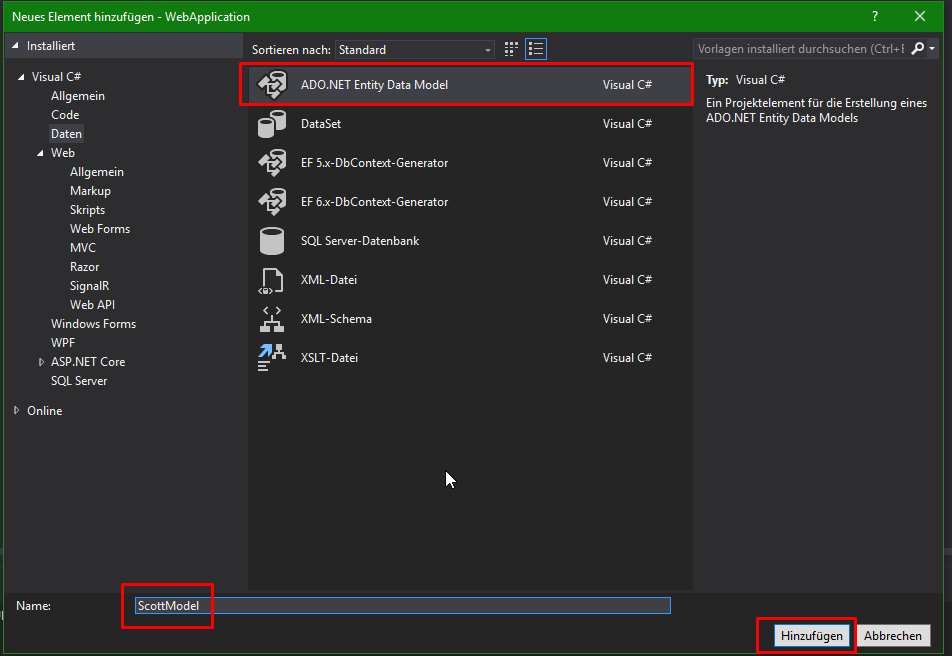
\includegraphics[width=\textwidth]{Parser_EFUse04}
    \caption{ADO.NET Entity Data Model}
    \label{fig:parsef04}
\end{figure} 
Im nächsten Fenster nun  ''EF Designer aus Datenbank'' auswählen und ''Weiter''
\begin{figure}[H]
    \centering
    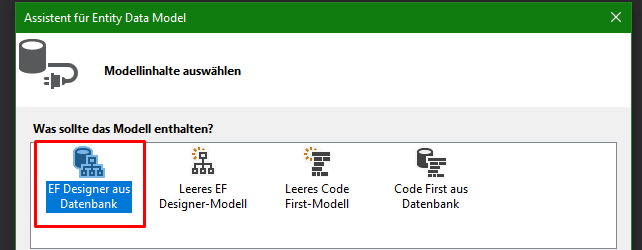
\includegraphics[width=\textwidth]{Parser_EFUse05}
    \caption{EF Designer aus Datenbank}
    \label{fig:parsef05}
\end{figure} 
Hier zunächst die Verbindung auswählen in diesem Fall ist ein lokales Datenbankfile vorhanden, daher wird dieses per DropDownMenü ausgewählt und auf ''Weiter''
\begin{figure}[H]
    \centering
    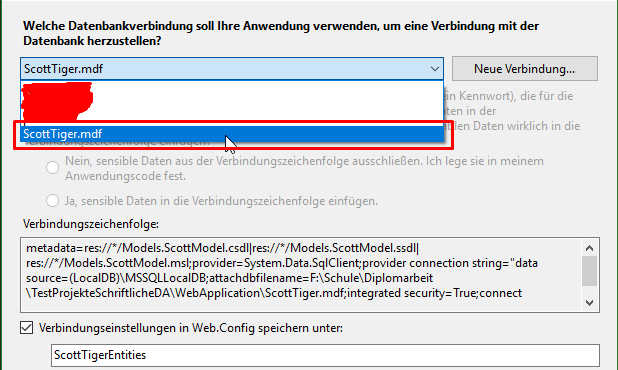
\includegraphics[width=\textwidth]{Parser_EFUse06}
    \caption{Datenverbindung}
    \label{fig:parsef06}
\end{figure} 
Alle Tabellen auswählen und auf ''Fertig stellen''. 
\begin{figure}[H]
    \centering
    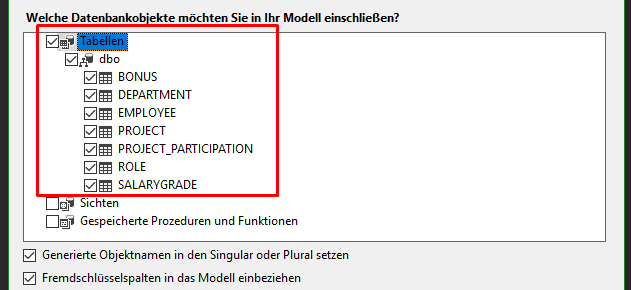
\includegraphics[width=\textwidth]{Parser_EFUse07}
    \caption{Datenbankobjekte auswählen}
    \label{fig:parsef07}
\end{figure} 
Falls eine Sicherheitswarnung erscheint auf ''OK'' klicken. \\
Endresultat, das Entity Framework hat die Tables im Models Ordner erstellt und am Bildschirm sieht man das Klassen mit ihren Beziehungen. Dies sollte ungefähr so aussehen:
\begin{figure}[H]
    \centering
    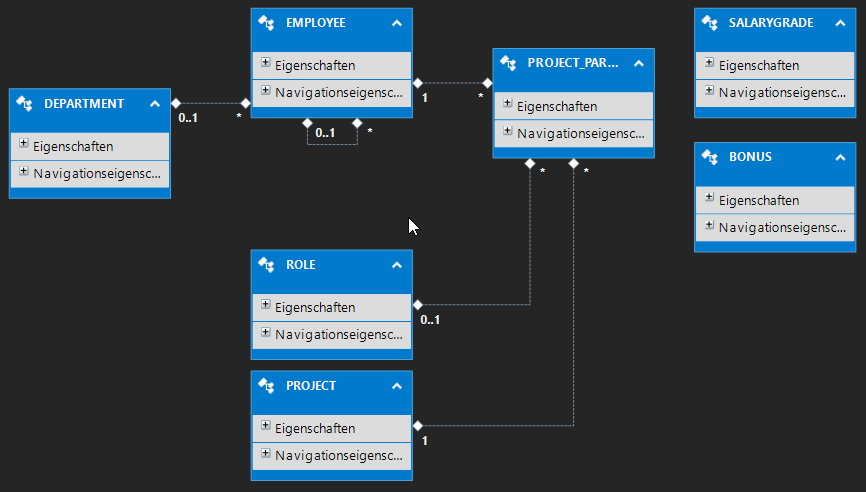
\includegraphics[width=\textwidth]{Parser_EFUse09}
    \caption{Klassendiagramm}
    \label{fig:parsef07}
\end{figure} 
\begin{figure}[H]
    \centering
    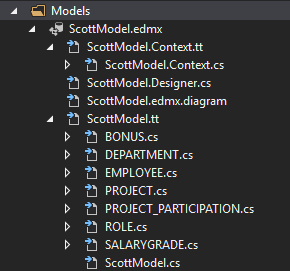
\includegraphics[width=0.5\textwidth]{Parser_EFUse10}
    \caption{Solutionsexplorer}
    \label{fig:parsef07}
\end{figure} 



\subsubsection{Source-Code}
\label{ef-sourcecode}
%Hier kommt die Source-Code Erklärung des Parsers hin

%SOURCE CODE VOM iCalContext
%	 public virtual DbSet<ActionTable> ActionTable { get; set; }
%    public virtual DbSet<Alarm> Alarm { get; set; }
%    public virtual DbSet<Attendance> Attendance { get; set; }
%    public virtual DbSet<Attendee> Attendee { get; set; }
%    public virtual DbSet<AttendeeAlarm> AttendeeAlarm { get; set; }
%    public virtual DbSet<Calendar> Calendar { get; set; }
%    public virtual DbSet<CalendarClass> CalendarClass { get; set; }
%    public virtual DbSet<CalendarEntry> CalendarEntry { get; set; }
%    public virtual DbSet<EventTable> EventTable { get; set; }
%    public virtual DbSet<Frequency> Frequency { get; set; }
%    public virtual DbSet<Organizer> Organizer { get; set; }
%    public virtual DbSet<Partstat> Partstat { get; set; }
%    public virtual DbSet<RoleTable> RoleTable { get; set; }
%    public virtual DbSet<Rrule> Rrule { get; set; }
%    public virtual DbSet<StatusTable> StatusTable { get; set; }
%    public virtual DbSet<TimeZone> TimeZone { get; set; }
%    public virtual DbSet<Todo> Todo { get; set; }
%    public virtual DbSet<TriggerTable> TriggerTable { get; set; }
%    public virtual DbSet<UserHasCalendar> UserHasCalendar { get; set; }
%    public virtual DbSet<UserTable> UserTable { get; set; }

%	protected override void OnModelCreating(ModelBuilder modelBuilder)
%    {
%      modelBuilder.Entity<ActionTable>(entity =>
%      {
%        entity.HasKey(e => e.ActionId);
%
%        entity.Property(e => e.ActionId).ValueGeneratedNever();
%
%        entity.Property(e => e.ActionName)
%                  .IsRequired()
%                  .HasMaxLength(50);
%      });
